\documentclass[11pt]{article}
\usepackage[margin=2.54cm]{geometry}
\usepackage[colorlinks,urlcolor=blue]{hyperref}
\usepackage{url}
\usepackage{graphicx}

\usepackage{enumitem}
\setlist[enumerate,1]{start=0} % only outer nesting level

\title{Classifying Movie Genres With Plot Summaries}
\author{Brian Kimmig, Jesus Zarate}
\date{}

\begin{document}

\maketitle

\section{Introduction}
\label{sec:introduction}

The internet today contains an abundance of information. We see a great deal of images, videos, and somewhat more abundant, text. It is a common problem for people to want to summarize a topic or the content of a chunk of text. This is a challenging problem for computers and machine learning (ML) algorithms as sentences and paragraphs are highly unstructured. A majority of ML algorithms require the data to be in a consistent form, vectors and matrices. Furthermore, they require that the data is numerical. This poses the main problem for us, how do you meaningfully turn a sentence, paragraph, or chunk of text into numerical data?

The goal of this project was to take text data, and assign it to a category (or categories). We could try to do this with Twitter data but the categorizing of Tweets can be largely subjective and was beyond the scope of this class. We decided that a good dataset to try these methods on would be film synopses and genres. In this case the text describing a movie can vary greatly, but there is a consistent and widely agreed on genre categorization. This makes for a great dataset to help us see if we can categorize textual data. We aim to see if we can take the text of a film synopses, build meaningful features, and learn a model to categorize the genres of other movies based on their synopses. 

\section{Data}
\label{sec:data}

We obtained the base of our data from a dataset published on \href{https://www.kaggle.com/deepmatrix/imdb-5000-movie-dataset}{Kaggle}. The dataset contained information on $\sim5000$ movies. We used this dataset for the movie list and the IMDB IDs. With IMDB IDs it is easy to automate gathering the synopses of each movie via GET requests to the \href{https://www.omdbapi.com/}{OMDB API}. The OMDB API allows you to search for movies, and gather information via the title or the IMDB ID. To ensure we get the correct information for every movie we performed GET requests querying with the IMDB ID. 

The OMDB API allows a user to specify the length of the plot summary it returns, with either 'full' or 'short'. We chose to gather the 'full' synopses for every movie we queried.

From the Kaggle data we used the OMDB API to compile title, plot summary, and genres for all $\sim5000$ movies. The data was stored in a JSON file, with each entry (or movie) containing the fields ['title', 'plot', 'genres'].

There were considerably more genres than expected, in total there were 26. Figure \ref{fig:genres} shows every genre and its percent occurrence. In our data, there were genres that occurred less than 1\% of the time, and generally they tended to be more obscure genres. Specifically, the genre 'Game-Show' occurred 0.02\% of the time. Because of the rare genres we decided to limit our genre classification labels to those that occur more often. In the end we settled on a cut of 10\% (shown by the red dotted line in Figure \ref{fig:genres}). This was to ensure that we had captured the major, or most common, genres. The cut of 10\% also ensured that every movie had at least 1 label, or genre, associated with it. If the cut was higher, we found that some movies did not have a genre associated with it. We also wanted to avoid throwing away data. 

\begin{figure}[ht]
	\centering
		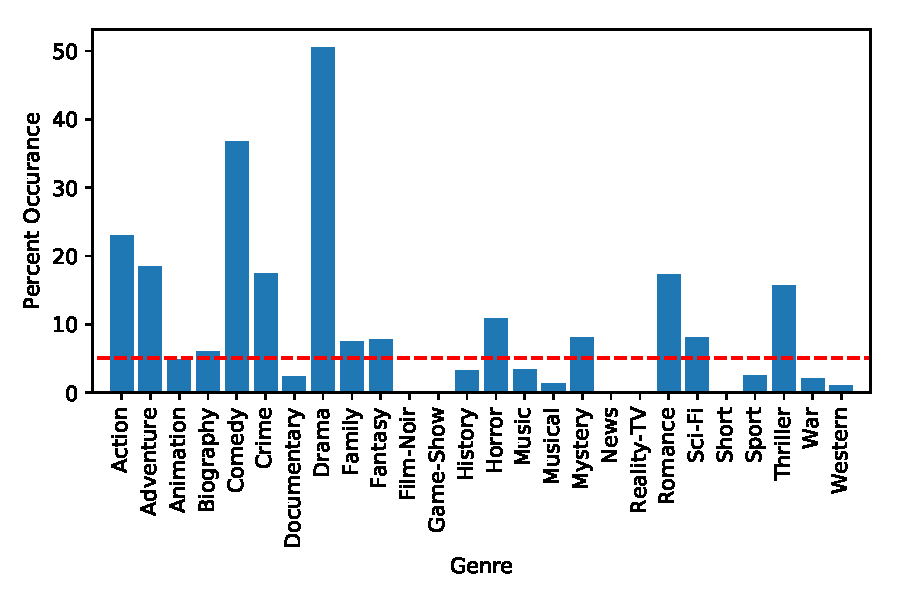
\includegraphics[width=0.5\textwidth,height=5cm]{genres.pdf}
	\caption{The percent occurrence for each genre. The red dotted line represents the cut made to get the list of genres (10\%).}
	\label{fig:genres}
\end{figure}

In the end, with our 10\% cut we ended up with the genres Action, Adventure, Comedy, Crime, Drama, Horror, Romance, and Thriller.

The genre labels set up with a one hot encoding. This was done to allow us to easily classify them with either a multi label classifier, or by individually, by column, with other classifiers (discussed further in \S \ref{sec:methods}). 

% Figure \ref{fig:one_hot} shows the genres for every movie in the one hot encoding. A yellow line indicates the movie is associated with that genre, from this we can clearly see that a majority of the movies are associated with the 'Drama' genre.

% \begin{figure}[ht]
% 	\centering
% 		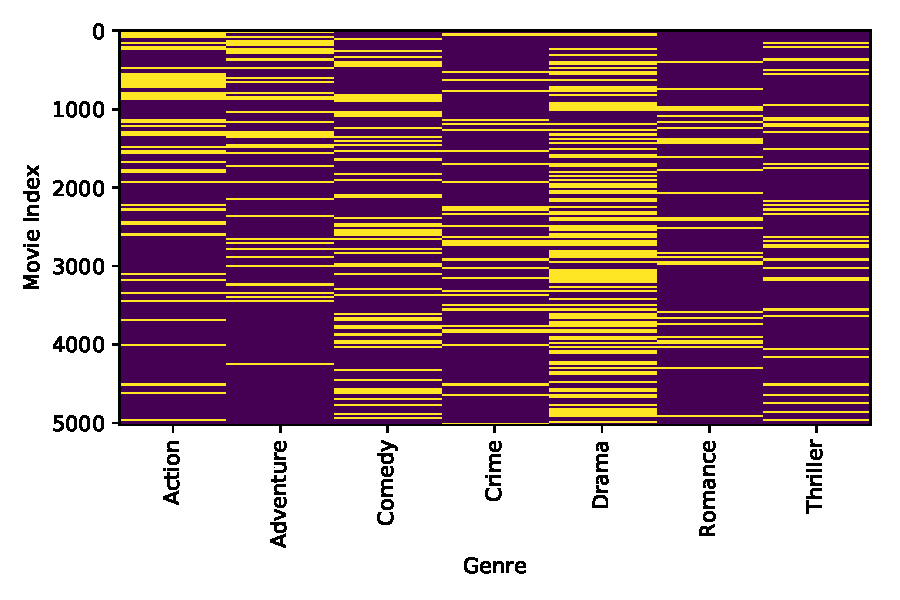
\includegraphics[width=0.75\textwidth]{one_hot_genres.pdf}
% 	\caption{The one hot encoding of the genres for every movie. Each row represents a movie and a column represents a genre. Yellow indicates the movie has that genres associated with it.}
% 	\label{fig:one_hot}
% \end{figure}

The synopses of the movies live in long strings or documents. We have a list of these that we will processing to create the features that we will then use to build models to classify genres. Extracting features from these documents is the main part of the project and will be discussed \S \ref{sec:methods}.

\section{Methods and Results}
\label{sec:methods}

In this section we will discuss the methods we used to create features for classification. We will start by creating features using Term Frequency - Inverse Document Frequency (TF-IDF), then with Latent Dirichlet Allocation \cite{blei2003}, and finally a combination of the two. 

We will classify genres of movies with three different classifiers. The first will be a simple linear regression, as learned in class. The labels are binary for each genre, so some thresholding will be done to get labels using linear regression. Next, we will classify with logistic regression, which is a well known regression model for predicting binary labels. For both linear and logistic regression we will fit for each genre individually. The last classifier we use will be the random forest \cite{breiman2001}. We chose to use Random Forests due to their popularity in data science competitions and their multi label classification capabilities; we can classify all labels simultaneously. 

For both the logistic regression, and random forest classifier we used the scikit-learn implementations \cite{scikit-learn}.

For classification, we randomly split our data into a test and a train set. The test size was 40\% of the data leaving the train with 60\%. In the following subsections we fit with the train data and check our answers with the test data. The F1-scores noted below were calculated from the test data. We would like to note that just creating a uniform random matrix of 0s and 1s gives an average score of $\sim0.3$.

\subsection{Term Frequency - Inverse Document Frequency}
\label{sec:tfidf}

To create the feature matrix we used {\it Term Frequency - Inverse Document Frequency} \href{https://en.wikipedia.org/wiki/Tf\%E2\%80\%93idf}{(TF-IDF)}, which is a similar idea to $k$-grams, but with small differences.  This looks at how frequently a term occurs in a document, in this case a movie synopsis, in combination with how frequently it occurs across all of the documents. This effectively down-weights the words that occur frequently in all documents. The term frequency is the number of times a given $k$-gram occurs in a document, and the inverse document frequency is the number of documents divided by the number of documents in which the $k$-gram occurs (the log of this is generally taken). First we create the matrix of term frequency counts represented in matrix form with $k$-grams as columns and each movie as a row. The inverse document frequency is a vector that contains the IDF for each $k$-gram. The final feature matrix is the multiplication of each TF row by the IDF vector.

The next step is to get rid of common words. The first thing we did was try to eliminate stop words by just removing them from the columns of the matrix. \href{https://en.wikipedia.org/wiki/Stop_words}{Stop words} generally refer to the most common words in a language and will most likely not provide useful information in our feature matrix. However, removing stop words was not good enough, since we still had too many features.  Therefore we decided to eliminate items that did not provide good information. We did this by making a cut on the document frequency, meaning that we didn't want words that were common in a given percentage of the documents.

% Although, TF-IDF was able to help us with eliminating the words or $k$-grams that do not give us information by making a cut on the inverse document frequency, we decided to make the cut on just the document frequency. 

To this point, we have created the TF-IDF sparse matrix using single words and a cut on the document frequency at 70\%. This gave us a sparse matrix of shape $5029 \times 23988$ (rows by columns) with 234,707 elements. At this point 23988 features is too many features, and most of those features might not provide any useful information, so we decided to use PCA in order to get the things that provide the most useful information. We experimented on few different number of features in order to see if there was more useful information in the data that we need to consider. 

% We then split this data into a train and test samples, with the test portion being 40\% of the data. 

%We trained the basic out of the box \href{http://scikit-learn.org/stable/modules/generated/sklearn.ensemble.RandomForestClassifier.html}{Random Forest Classifier} from scikit-learn. 

\begin{figure}[ht]
	\centering
		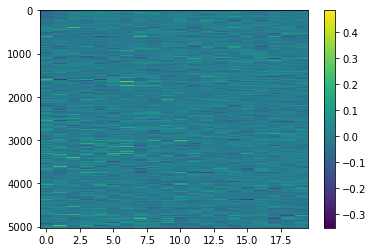
\includegraphics[width=0.5\textwidth,height=5cm]{TF-IDF.png}
	\caption{The feature matrix generated using TF-IDF. The rows represent each movie and the columns represent the topic number reduced to 20 features using PCA}
	\label{fig:tfidf}
\end{figure}

\label{sec:tfidf}

\subsubsection{Linear Regression}

In this section we used Least squares classifying one genre at a time, with TF-IDF and different features using PCA. We tested 5 values in order to see which values gave us the best results with the least amount of features. From 20 to 500 features we can see an increasingly better average, but by increasing the features by 500 the average actually decreases. At this point we can tell that a "sweet spot" of features is right around 500. Table \ref{tab:lr_scores} contains the scores for each genre based on the number of principal components used.

\begin{table}[h]
	\label{tab:lr_scores}
\begin{center}
	\begin{tabular}{| l | l | l | l | l | l |}
		\hline		         
                  & PCA 20    & PCA 200           & PCA 500     & PCA 1000  & PCA 2000 \\\hline
        Genre     & F1-Score  & F1-Score          & F1-Score    & F1-Score  & F1-Score\\\hline		
	  	Action    & 0.45      & 0.57 			  & 0.58        & 0.56      &  0.46\\
		Adventure & 0.37      & 0.53 			  & 0.54        & 0.53      &  0.41\\
		Comedy    & 0.27      & 0.46 			  & 0.27        & 0.48      &  0.22\\
		Crime     & 0.42      & 0.56 			  & 0.57        & 0.55      &  0.43\\
		Drama     & 0.21      & 0.40 			  & 0.45        & 0.44      &  0.44\\
		Horror    & 0.11      & 0.51 			  & 0.34        & 0.52      &  0.27\\
		Romance   & 0.37      & 0.47 			  & 0.34        & 0.42      &  0.24\\ 
		Thriller  & 0.08      & 0.33 			  & 0.45        & 0.37      &  0.32\\\hline
		Average   & 0.22      & 0.40 			  & 0.43        & 0.42      &  0.35\\\hline       
	\end{tabular} 
\end{center}
	\caption{F1-Scores for the top 20, 200, 500, 1000, 2000 principal components and Linear Regression model.}
\end{table}


\subsubsection{Logistic Regression}

Another regression technique we used was \href{https://en.wikipedia.org/wiki/Logistic_regression}{Logistic Regression}. It is a regression model that has a categorical dependent variable. The dependent variable can be a binary dependent variable, or in our case where the dependent variable has more than two categories multinomial logistic regression was used. The classification was done one genre at a time as well.

When we performed the same experiment as with linear regression, again there was a noticeable increase from 20 to 200, but from 500 to 2000 features the increase factor is very small, and therefore we can argue that the information on data above 500 is minimal, and we can ignore that data.

With Logic regression we can see that we do better than with linear regression. Table \ref{tab:logr_scores} contains the F1-Scores for varying number of principal components. 

\begin{table}[h]
	\label{tab:logr_scores}
\begin{center}
	\begin{tabular}{| l | l | l | l | l | l |}
		\hline		         
                  & PCA 20    & PCA 200           & PCA 500     & PCA 1000  & PCA 2000 \\\hline
        Genre     & F1-Score  & F1-Score          & F1-Score    & F1-Score  & F1-Score\\\hline		
	  	Action    & 0.58      & 0.68			  &  0.66       & 0.66     &  0.66\\
		Adventure & 0.43      & 0.48			  &  0.52       & 0.52     &  0.51\\
		Comedy    & 0.56      & 0.62			  &  0.63       & 0.63     &  0.63\\
		Crime     & 0.51      & 0.58			  &  0.60       & 0.60     &  0.62\\
		Drama     & 0.62      & 0.71			  &  0.69       & 0.71     &  0.72\\
		Horror    & 0.33      & 0.44			  &  0.48       & 0.48     &  0.48\\
		Romance   & 0.50      & 0.56			  &  0.59       & 0.59     &  0.59\\ 
		Thriller  & 0.38      & 0.40			  &  0.43       & 0.43     &  0.41\\\hline
		Average   & 0.396     & 0.452 			  & 0.469       & 0.469    &  0.47\\\hline       
	\end{tabular} 
\end{center}
	\caption{F1-Scores for the top 20, 200, 500, 1000, 2000 principal components and Logistic Regression model.}
\end{table}


\subsubsection{Random Forest}
Finally for this section we performed the same experiment on a \href{http://scikit-learn.org/stable/modules/generated/sklearn.ensemble.RandomForestClassifier.html}{Random Forest}, and we performed this classification on all genres at once. 

\begin{table}[h]
	\label{tab:randf_scores}
\begin{center}
	\begin{tabular}{| l | l | l | l | l | l |}
		\hline		         
                  & PCA 20    & PCA 200           & PCA 500     & PCA 1000  & PCA 2000 \\\hline
        Genre     & F1-Score  & F1-Score          & F1-Score    & F1-Score  & F1-Score\\\hline		
	  	Action    & 0.30     & 0.34		          & 0.28        & 0.29      & 0.28\\
		Adventure & 0.20     & 0.16		          & 0.19        & 0.21      & 0.23\\
		Comedy    & 0.47     & 0.47		          & 0.47        & 0.45      & 0.45\\
		Crime     & 0.21     & 0.29		          & 0.25        & 0.28      & 0.28\\
		Drama     & 0.67     & 0.68		          & 0.66        & 0.66      & 0.68\\
		Horror    & 0.13     & 0.13		          & 0.13        & 0.14      & 0.14\\
		Romance   & 0.24     & 0.23		          & 0.30        & 0.27      & 0.27\\ 
		Thriller  & 0.11     & 0.12		          & 0.13        & 0.10      & 0.14\\\hline
		Average   & 0.211     & 0.215 	          & 0.216       & 0.216     & 0.223 \\\hline       
	\end{tabular} 
\end{center}
	\caption{F1-Scores for the top 20, 200, 500, 1000, 2000 principal components and Random Forest model.}
\end{table}


\subsection{Latent Dirichlet Allocation}
\label{sec:lda}

Topic models are methods of taking large amounts of data and finding, understanding, and summarizing the information in it \cite{wiki:topic_model, kdnuggets:topic_model}. We believe that hidden in these plot summaries there will be some fairly obvious groups of words, or topics, that will be seen together. After some on-line research we came across the concept of Latent Dirichlet Allocation (LDA) \cite{blei2003}. LDA is a fairly popular topic model. 

LDA essentially looks for topics in documents, determines some topics, and gives an estimate of the proportion of that topic that is seen in the document. The general idea that documents are random mixtures of topics, and topics are characterized by words \cite{blei2003}. 

In a basic sense, LDA works by assigning random topics (the number of which is chosen by the user) to the words in each document. This gives you an initial representation of the topic distribution in each document. From there you can improve the distributions by sampling. Pick a word and a topic, then topic with probability proportional to p(topic$|$document) times p(word$|$topic) update that word to the new topic. The hope is that after some number of iterations the assignments will become stable (and something you agree with) \cite{kdnuggets:topic_model, chen2011, blei2003}. 

We discovered this method later and did not have time to write a full routine for this. Therefore, we chose to use a the LDA routine in scikit-learn \cite{scikit-learn}. This implementation allows you to pick the number of topics you would like created and lets you tweak and set some other parameters. We chose to use the default settings for everything but the number of topics. We chose the number of topics to be equal to the number of genres. We did this to see if the words in the topics found matched with those of the genres. Below you can see the topics, by number, and the top 20 words associated with that topic.

{\small
\begin{enumerate}
\setlength\itemsep{0.0em}

\item professor king prince princess invention ma queen oil england throne bennett land lord east coast tournament royal chinese lily pakistan

\item new york city family world life story school money young film lives harry team american students ray real follows mind

\item earth group evil years human world alien crew planet save ship team son race los angeles help time michael new

\item life man young family father old love mother woman story town year years time finds help son daughter home lives

\item war police world agent murder group killer drug team american secret mission bond case man fbi detective forces government president

\item alex lee danny hannah winter wilderness julie bent guide lion scam pat pearl lizzie rush hughes black hole various irving

\item school friends life high friend best love new night day college big movie just sex star gets girl time party

\item charlie victor darkness experiments bridge madness wallace matrix exorcism tried australia el khan horrifying andrea neo jamal melanie frankenstein trainer
\end{enumerate}
}

We see that some of the words in the topics are kind of ambiguous, but in some cases the topics seem to be distinguishable. For instance, in topic 4 we see words that may fit well with the topic 'Crime', and in topic 7 we see words that fit well in the 'Horror' category. In topic 3, we see words that could likely be found describing a 'Drama'.

The feature matrix obtained from LDA is very different from that of TF-IDF. Each movie gets a distribution over topics, meaning each movie has some percentage of each topic. Figure \ref{fig:lda} shows the final feature matrix that will be used to classify genres. In Figure \ref{fig:lda} there are clearly topics that are more prominent than others, specifically topic \#3. In comparison to Figure \ref{fig:tfidf} there seems to be much more coherent structure in the LDA feature matrix (Figure \ref{fig:tfidf}).

\begin{figure}[ht]
	\centering
		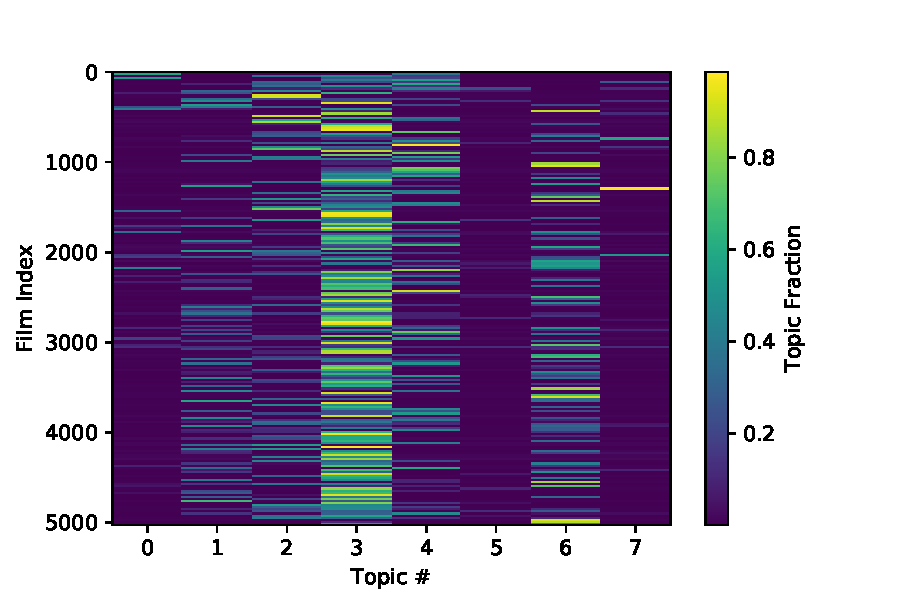
\includegraphics[width=0.5\textwidth,height=5cm]{lda_features.pdf}
	\caption{The feature matrix generated using LDA. The rows represent each movie and the columns represent the topic number. Each row sums to 1. The topic fraction for each movie is represented by the color. For this we specified 8 topic. We can clearly see that some topics (2, 3, 4, 6) are more prevalent than others.}
	\label{fig:lda}
\end{figure}

Finally, we fit the data. Table \ref{tab:lda_scores} shows the scores for every category. For this set of features both the linear regression and the logistic regression do a better job than the random forest. However, we would like to note that this could be due to poor parameter tuning on the random forest.

\begin{table}[h]
	\label{tab:lda_scores}
\begin{center}
	\begin{tabular}{| l | l | l | l |}
		\hline
		           & Linear Regression & Logistic Regression & Random Forest \\
		\hline
		Genre      & F1-Score          & F1-Score            & F1-Score       \\
	  	\hline			
	  	Action     & 0.58              & 0.57                & 0.42 \\
	  	Adventure  & 0.42              & 0.42                & 0.25 \\ 
	  	Comedy     & 0.59              & 0.54                & 0.47 \\
	  	Crime      & 0.38              & 0.42                & 0.17 \\
	  	Drama      & 0.67              & 0.65                & 0.57 \\
	  	Horror     & 0.09              & 0.23                & 0.16 \\
	  	Romance    & 0.42              & 0.41                & 0.21 \\
	  	Thriller   & 0.28              & 0.34                & 0.19 \\
	  	\hline
	  	Average    & 0.43              & 0.44                & 0.30 \\
	  \hline  
	\end{tabular}
\end{center}
	\caption{The F1 scores for the prediction of each genre using LDA to generate features. The last row indicates the average. The random forest classifier, on average, does as well as guessing.}
\end{table}

\subsection{TF-IDF + LDA}
\label{sec:tfidf_lda}

In this section we decided to see if we can improve our classifications by combining the TF-IDF features with the features from LDA. Obviously we won't want to use every feature from TF-IDF, as there can be thousands of columns, so we will use PCA to get the top 200 components. Table \ref{tab:lda_tfidf_scores} shows the scores for each genre and the average score. In general, the scores all increased with the this collection of features. 

\begin{table}[h]
	\label{tab:lda_tfidf_scores}
\begin{center}
	\begin{tabular}{| l | l | l | l |}
		\hline
		           & Linear Regression & Logistic Regression & Random Forest \\
		\hline
		Genre      & F1-Score          & F1-Score            & F1-Score       \\
	  	\hline			
	  	Action     & 0.63              & 0.63                & 0.31 \\
	  	Adventure  & 0.55              & 0.53                & 0.17 \\ 
	  	Comedy     & 0.62              & 0.62                & 0.40 \\
	  	Crime      & 0.57              & 0.53                & 0.16 \\
	  	Drama      & 0.71              & 0.69                & 0.64 \\
	  	Horror     & 0.51              & 0.40                & 0.14 \\
	  	Romance    & 0.53              & 0.46                & 0.06 \\
	  	Thriller   & 0.43              & 0.43                & 0.13 \\
	  	\hline
	  	Average    & 0.57              & 0.54                & 0.25 \\
	  \hline  
	\end{tabular}
\end{center}
	\caption{The F1 scores for the prediction of each genre using LDA and TF-IDF to generate features. The last row indicates the average. The random forest classifier, on average, does slightly worse than guessing.}
\end{table}

\section{Discussion}
\label{sec:discussion}

In this project we compared numerous feature creation methods and classification methods. We found that both TF-IDF and LDA are useful tools for transforming textual data to structured data. In general, I think we were surprised with how much better the linear models did than the random forest; the random forest did no better than just randomly guessing. It is nice to see why these methods are so highly regarded. (We should note that the random forest may have eventually done better with classification if we did more parameter tuning, as it is highly dependent on that.)

There is predictive power in both the features generated using TF-IDF and LDA. It was helpful to see an improvement in prediction when combining the methods. We found that some of the hardest parts data mining and feature creation came from trying to figure out what gives good predictive power. We would be interested to see if other parameters, possibly not in the text, help us build better models. In the end we found that classifying text is a very difficult task. Even at our best we were not much better than just guessing randomly.

\bibliography{bibliography}{}
\bibliographystyle{plain}

\end{document}

% \begin{table}[h]
% 	\label{tab:genres}
% \begin{center}
% 	\begin{tabular}{| l | l |}
% 		\hline
% 		Genre & \% Occurrence \\
% 		\hline
% 		Action & 23.007\% \\
% 	  \hline  
% 	\end{tabular}
% \end{center}
% 	\caption{}
% \end{table}
